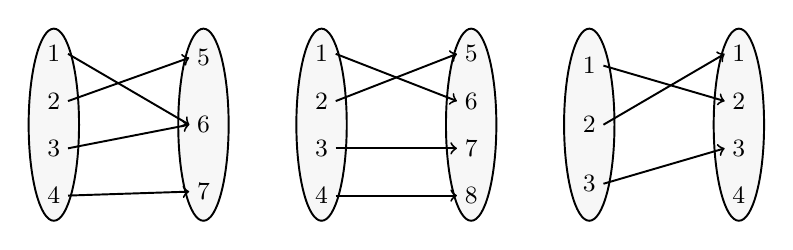
\begin{tikzpicture}[line width=.7pt,
  every node/.style={font=\small,inner sep=0pt}]
% Surjective, but not injective: 1 and 3 both map to 6.
\begin{scope}
  \filldraw[fill=black!3] (.3,0) ellipse[x radius=.32,y radius=1.22];
  \filldraw[fill=black!3] (2.2,0) ellipse[x radius=.32,y radius=1.22];
  \foreach \n/\y in {1/.9,2/.3,3/-.3,4/-.9}
    \node at (.3,\y) {$\n$};
  \foreach \n/\y in {5/.85,6/0,7/-.85}
    \node at (2.2,\y) {$\n$};
  \draw[->] (.48,.9)--(2.02,0);
  \draw[->] (.48,.3)--(2.02,.85);
  \draw[->] (.48,-.3)--(2.02,0);
  \draw[->] (.48,-.9)--(2.02,-.85);
\end{scope}
% Bijective.
\begin{scope}[xshift=3.4cm]
  \filldraw[fill=black!3] (.3,0) ellipse[x radius=.32,y radius=1.22];
  \filldraw[fill=black!3] (2.2,0) ellipse[x radius=.32,y radius=1.22];
  \foreach \n/\y in {1/.9,2/.3,3/-.3,4/-.9}
    \node at (.3,\y) {$\n$};
  \foreach \n/\y in {5/.9,6/.3,7/-.3,8/-.9}
    \node at (2.2,\y) {$\n$};
  \draw[->] (.48,.9)--(2.02,.3);
  \draw[->] (.48,.3)--(2.02,.9);
  \draw[->] (.48,-.3)--(2.02,-.3);
  \draw[->] (.48,-.9)--(2.02,-.9);
\end{scope}
% Injective, but not surjective: 4 is not an output.
\begin{scope}[xshift=6.8cm]
  \filldraw[fill=black!3] (.3,0) ellipse[x radius=.32,y radius=1.22];
  \filldraw[fill=black!3] (2.2,0) ellipse[x radius=.32,y radius=1.22];
  \foreach \n/\y in {1/.75,2/0,3/-.75}
    \node at (.3,\y) {$\n$};
  \foreach \n/\y in {1/.9,2/.3,3/-.3,4/-.9}
    \node at (2.2,\y) {$\n$};
  \draw[->] (.48,.75)--(2.02,.3);
  \draw[->] (.48,0)--(2.02,.9);
  \draw[->] (.48,-.75)--(2.02,-.3);
\end{scope}
\end{tikzpicture}
